%(BEGIN_QUESTION)
% Copyright 2006, Tony R. Kuphaldt, released under the Creative Commons Attribution License (v 1.0)
% This means you may do almost anything with this work of mine, so long as you give me proper credit

Følgende sløyfediagram viser et anti-surge-reguleringssystem for kompressor. Når strømningsregulatoren (FIC 42) oppdager høy differansetrykk over kompressoren samtidig med lav strømning gjennom kompressoren, åpner den surge-ventilen (FV 42), slik at strømning bypasses fra kompressorutløpet tilbake til kompressorinnløpet:

$$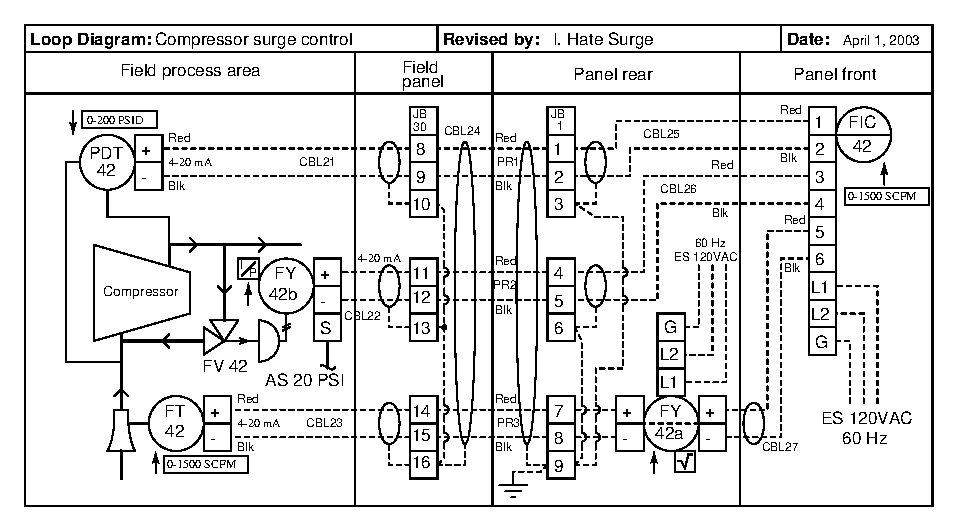
\includegraphics[width=15.5cm]{i00134x01.eps}$$

Hvis skruen på terminal JB1-4 løsner, slik at forbindelsen mellom de to ledningene i dette punktet brytes, hva vil surge-ventilen gjøre, og hvilken effekt tror du det vil ha på kompressoren?

\vskip 20pt \vbox{\hrule \hbox{\strut \vrule{} {\bf Forslag til sokratisk diskusjon} \vrule} \hrule}

\begin{itemize}
\item{} Identifiser om FV-42 er {\it fail-open} (FO) eller {\it fail-closed} (FC).
\item{} Hva representerer de korte pilene (ved siden av instrumentboblene) i dette sløyfediagrammet?
\end{itemize}

\underbar{file i00134}
%(END_QUESTION)





%(BEGIN_ANSWER)

Hvis skruen på JB1-4 løsner, avbrytes strømmen til I/P-omformeren, og den pneumatiske utgangen feiler lavt. Vi vet dette fordi oppoverpilen ved FY-42b viser direktevirkende funksjon (mer mA = mer lufttrykk ut). Med lavt lufttrykk til bypassventilen vil ventilen feile åpen (som vist av pilen ved ventilspindelsymbolet). Da bypasses strømning fra utløp til innløp på kompressoren, og gassstrømmen til prosessen reduseres.

\vskip 10pt

Til informasjon: kompressorsurge er et fluiddynamisk fenomen der skovlene i en ikke-fortrengningskompressor (f.eks. aksial eller sentrifugal) «staller», på samme måte som flyvinger ved for lav fart og/eller for stor angrepsvinkel. Når skovlene staller, mister de «grep» på gassen, den mekaniske drivkilden avlastes (motor/turbin), kompressoren øker hastighet, skovlene «unstaller», og driveren belastes igjen. Deretter kan syklusen gjenta seg.

Følgende utdrag er hentet fra Francis Shinskeys bok {\it Energy Conservation and Control}, Academic Press, 1978, om kompressorsurge:

\vskip 10pt {\narrower \noindent \baselineskip5pt

``The most demanding aspect of controlling compressors is surge protection.  The problem lies in being unable to determine with absolute certainty the degree of approach to surge.  Once a compressor begins to surge, it will continue until corrective action is applied, so automatic protection is mandatory.  A small centrifugal compressor may surge several times without damage, but a 100,000-hp axial could require reblading after a single incident.''

\vskip 5pt

``When a compressor begins to surge, the suction flow falls to zero within a few milliseconds, reverses momentarily, and begins to recover in less than a half second.  If the situation is not corrected, the cycle repeats immediately, resulting in a series of thunderclaps less than a second apart.  The sudden fall in suction flow can be detected and used to open a recirculating valve, but not before at least one surge cycle is sustained.  To prevent surge from developing at all requires a control system which skirts the unstable area altogether.''

\par} \vskip 10pt

%(END_ANSWER)





%(BEGIN_NOTES)


%INDEX% Documentation, loop diagram: compressor surge control
%INDEX% Documentation, loop diagram: fault analysis

%(END_NOTES)
